\fancyhead[C]{\textit{Solutions}}

\section{Solutions to Section 1}
	\begin{table}[!h]
		\centering
		\begin{tabular}{c@{\hspace{2.5em}}cp{0.75\textwidth}}
			true & false & \\
			\specialrule{\lightrulewidth}{0.25em}{1.25em}
			\bubble & \dbubble & If \(Q \colon \mathbb{R}^n \to \mathbb{R},\) \(\vec{x} \mapsto \vec{x}^TA\vec{x}\) is a postive-definite quadratic 
						      form, then the largest eigenvalue of the matrix \(A\) is the largest value the quadratic form takes. \\[0.75em]
			\bubble & \dbubble & If the smallest singular value of \(A\) is 2, then the quadratic form \(Q(\vec{x}) = \|A\vec{x}\|^2 - \|\vec{x}\|^2\) is
						      indefinite. \\[0.75em]
			\dbubble & \bubble & If \(P \in \mathbb{R}^{m \times m}\) is an orthogonal matrix, then \(A \in \mathbb{R}^{m \times n}\) and 
						     \(PA\) have the same singular values. \\[0.75em]
			\bubble & \dbubble & If \(A \in \mathbb{R}^{n \times n}\), then \(\det A\) is the product of its singular values. \\[0.75em] 
			\dbubble & \bubble & If \(\det A = 3\) and \(A \in \mathbb{R}^{2 \times 2}\), then any linearly independent set of 2 vectors in 
						      \(\mathbb{R}^2\) form a basis for \(\colspace A\). \\[0.75em]
			\bubble & \dbubble & For row-equivalent matrices \(A, B \in \mathbb{R}^{m \times n}\), if \(A\vec{x} = \vec{b}\) is consistent then so is
						      \(B\vec{y} = \vec{b}\) for \(\vec{b} \in \mathbb{R}^m\), \(\vec{y}, \vec{x} \in \mathbb{R}^n\).\\[0.75em]
			\bubble & \dbubble & If \(A \in \mathbb{R}^{n \times n}\) has no zero entries, then \(\colspace A = \mathbb{R}^n\). \\[0.75em]
			\bubble & \dbubble & If \(\det A = 0\) then \(A\) has a row of 0s and \(A\vec{x} = \vec{b}\) is inconsistent for some 
						      \(\vec{b} \in \mathbb{R}^m\). \\[0.75em]
			\dbubble & \bubble & Not all lines in \(\mathbb{R}^2\) are subspaces. \\[0.75em]
			\bubble & \dbubble & If \(A, B \in \mathbb{R}^{n \times n}\) and \(T_A\) scales a region in \(\mathbb{R}^n\) by twice the amount 
						      \(T_B\) does, then \(\det(A) > \det(B)\). \\[0.75em]
			\dbubble & \bubble & If \(\{\vec{v}_1, \vec{v}_2, \vec{v}_3\}\) forms a basis for a subspace, then 
						      \(\{\vec{v}_1, \vec{v}_2 + \vec{v}_3, \vec{v}_1 + \vec{v}_3\}\) forms a basis for the same subspace.\\[0.75em]
			\bubble & \dbubble & Any two linearly independent vectors span \(\mathbb{R}^2.\) \\[0.75em]
			\dbubble & \bubble & If \(\{\vec{v}_1, \vec{v}_2, \vec{v}_3\}\) is orthogonal set in \(\mathbb{R}^3\) and 
						     \(W = \vspan\{\vec{v}_1, \vec{v}_3\}\), then \(W^\perp = \vspan\{2\vec{v}_2, \vec{v}_2\}\). \\[0.75em]
			\dbubble & \bubble & If \(\{\vec{v}_1, \vec{v}_2\}\) forms an orthonormal set, then \(\|\vec{v}_1 + \vec{v}_2\| = \sqrt{2}\). \\[0.75em]
			\dbubble & \bubble & If \(A \in \mathbb{R}^{2 \times 2}\) and \(A\) has a complex eigenvalue \(\lambda_1 = a + bi\), 
						      then \(\lambda_1\lambda_2 = a^2 + b^2\). \\[0.75em]
			\bubble & \dbubble & If a vector \(\vec{y} \in \mathbb{R}^n\) is expressed as \(\vec{u} + \vec{v}\), where \(\vec{v} \cdot \vec{u} = 0\), 
						      and \(\vec{u} \in \mathcal{W}\), then \(\vec{v}\) is \(\proj_\mathcal{W} \vec{y}\). \\[0.75em]
			\bubble & \dbubble & With \(A = A^T\), any two linearly independent eigenvectors \(\vec{v}_1, \vec{v}_2\) of \(A\) yield 
						     \(\vec{v}_1 \cdot \vec{v}_2 = 0\).\\[0.75em]
			\dbubble & \bubble & If \(\vec{\hat{v}}, \vec{\hat{u}}\) are least-square solutions to the equation \(A\vec{x} = \vec{b},\) then 
						      \(\vec{\hat{v}} - \vec{\hat{u}} \in \nullspace A\).\\[0.75em]
			\bubble & \dbubble & In \(LU\)-factorization of a square matrix \(A\), \(\det(A) = \det(U)\) and so the diagonal entries of \(U\) are the 
						      eigenvalues of \(A\). \\[0.75em]
			\bubble & \dbubble & The \(PDP^{-1}\) factorization of a matrix \(A \in \mathbb{R}^{n \times n}\) is unique. \\[0.75em]
			\dbubble & \bubble & If \(\{\vec{a}_1, \dots, \vec{a}_k\}\) is a basis for a subspace, and 
						      \(\{\vec{u}_1, \dots, \vec{u}_k\}\) is the result of the Gram-Schmidt process, then 
						     \(\vspan \{\vec{a}_1, \dots, \vec{a}_k\} = \vspan\{\vec{u}_1, \dots, \vec{u}_k\}\). \\[0.75em]
			\bottomrule
		\end{tabular}
	\end{table}


\section{Solutions to Section 2}
	\begin{table}[!h]
		\centering
		\begin{tabular}{c@{\hspace{2.5em}}cp{0.75\textwidth}}
			possible & impossible & \\
			\specialrule{\lightrulewidth}{0.25em}{1.25em}
			\bubble & \dbubble & A linear transformation \(T \colon \mathbb{R}^3 \to \mathbb{R}^2\) where the transformation is onto and the 
						      columns of the standard matrix \(A\) are linearly independent. \\[0.75em]
			\bubble & \dbubble & A matrix \(A\) with the property that \(A^TA\) has negative eigenvalues. \\[0.75em]
			\dbubble & \bubble & An orthogonal matrix \(U \in \mathbb{R}^{n \times n}\) whose determinant is not 1. \\[0.75em]
			\bubble & \dbubble & A diagonalizable matrix \(A \in \mathbb{R}^{n \times n}\) with the sum of its eigenvalues' geometric multiplicities 
						      being less than \(n\). \\[0.75em]
			\bubble & \dbubble & A regular stochastic matrix that has a column of zeroes. \\[0.75em]
			\bubble & \dbubble & A nonzero vector \(\vec{u}\) with \(\vec{u} \in \nullspace A\) and \(\vec{u} \in \colspace A^T\) for some real matrix 
						     \(A\). \\[0.75em]
			\bubble & \dbubble & A real matrix \(A \in \mathbb{R}^{n \times n}\) that is row equivalent to the identity matrix and there exists vectors 
						     \(\vec{x}, \vec{y} \in \mathbb{R}^n\) such that \(\vec{x} \ne \vec{y}\) and \(A\vec{x} = A\vec{y}\). \\[0.75em]
			\bottomrule
		\end{tabular}
	\end{table}
	
\section{Solutions to \textit{Fill in the Blank Questions}}
	\begin{enumerate}
		\item \(\sqrt[3]{\mathbf{4}}\).
		\item \(\mathbf{4}\).
		\item \(\mathbf{3}\).
		\item \(\mathbf{2}\).
		\item \(\begin{pmatrix}-1 \\ -2 \\ 5\end{pmatrix}\).
	\end{enumerate}

\section{Solutions to \textit{Construction Questions}}
	\begin{enumerate}
		\item We need to find a \(2 \times 3\) matrix whose columns are orthogonal to \(\begin{pmatrix}1 \\ 2\end{pmatrix}\). An example could be 
			 \[\begin{bmatrix}-2 & -2 & -2\\ 1 & 1 & 1\end{bmatrix}.\]
		\item A simple example could be \(\begin{bmatrix}1 & 0 \\ 0 & 0\end{bmatrix}\).
		\item Since \((\rowspace A)^\perp = \nullspace A\), if we have a focus on one of the restrictions, then we satisfy the other restriction. For example,
			the matrix \(\begin{bmatrix}-2 & 1 & 2\end{bmatrix}\) fullfills the rowspace requirement. However, it also \emph{automatically} fullfills the
			nullspace requirement. There's no limit on the number of rows as they could be constant multiplis of the given vector. However, there is a 
			constraint on the number of columns.
		\item \(\begin{bmatrix}2 & 0 & 0 \\ 0 & 1 & 1 \\ 0 & 0 & 1\end{bmatrix}\).
	\end{enumerate}

\section{Solutions to \textit{Short Answers}}
\begin{enumerate}
	\item 
	\[\begin{bmatrix}1 & -1 \\ 0 & 0 \\ 1 & -1\end{bmatrix} = \underbrace{\begin{bmatrix}1/\sqrt{2} & 0  & -1/\sqrt{2} \\ 0 & 1 & 0 \\ 1/\sqrt{2} & 0 & 1/\sqrt{2}\end{bmatrix}}_U \underbrace{\begin{bmatrix}2 & 0 \\ 0 & 0 \\ 0 & 0\end{bmatrix}}_\Sigma\underbrace{\begin{bmatrix}1/\sqrt{2} & -1/\sqrt{2} \\ 1/\sqrt{2} & 1/\sqrt{2}\end{bmatrix}}_{V^T}.\]
		\begin{enumerate}
			\item \(\left\{ \begin{bmatrix}1/\sqrt{2} \\ 0 \\ 1/\sqrt{2}\end{bmatrix} \right\}\).\footnote{In general, if \(\rank A = r\), then the first \(r\)
				 columns of \(U\) are form an orthonormal basis for the column space. The first \(r\) columns of \(V\) would also form an orthonormal
				 basis for \(\rowspace A\).}
			\item \(\left\{ \begin{bmatrix}1/\sqrt{2} \\ -1/\sqrt{2}\end{bmatrix} \right\}\).
			\item \(\left\{ \begin{bmatrix}1/\sqrt{2} \\ 1/\sqrt{2}\end{bmatrix} \right\}\).
			\item \(\max_{\|\vec{x}\| = 1} \|A\vec{x}\| = \sigma_1 = 2\). This value is attained when 
				\(\vec{x} = \pm\begin{bmatrix}1/\sqrt{2} \\ -1/\sqrt{2}\end{bmatrix}\).
			\item \(\min_{\|\vec{x}\| = 1} \|A\vec{x}\| = \sigma_2 = 0\). This value is attained when 
				\(\vec{x} = \pm\begin{bmatrix}1/\sqrt{2} \\ 1/\sqrt{2}\end{bmatrix}\).
		\end{enumerate}
	\item ~ %
		\begin{figure}[!h]
			\centering
			\begin{tabular}{c@{\hspace{2em}}c}
			\begin{minipage}{0.25\textwidth}
				\centering
				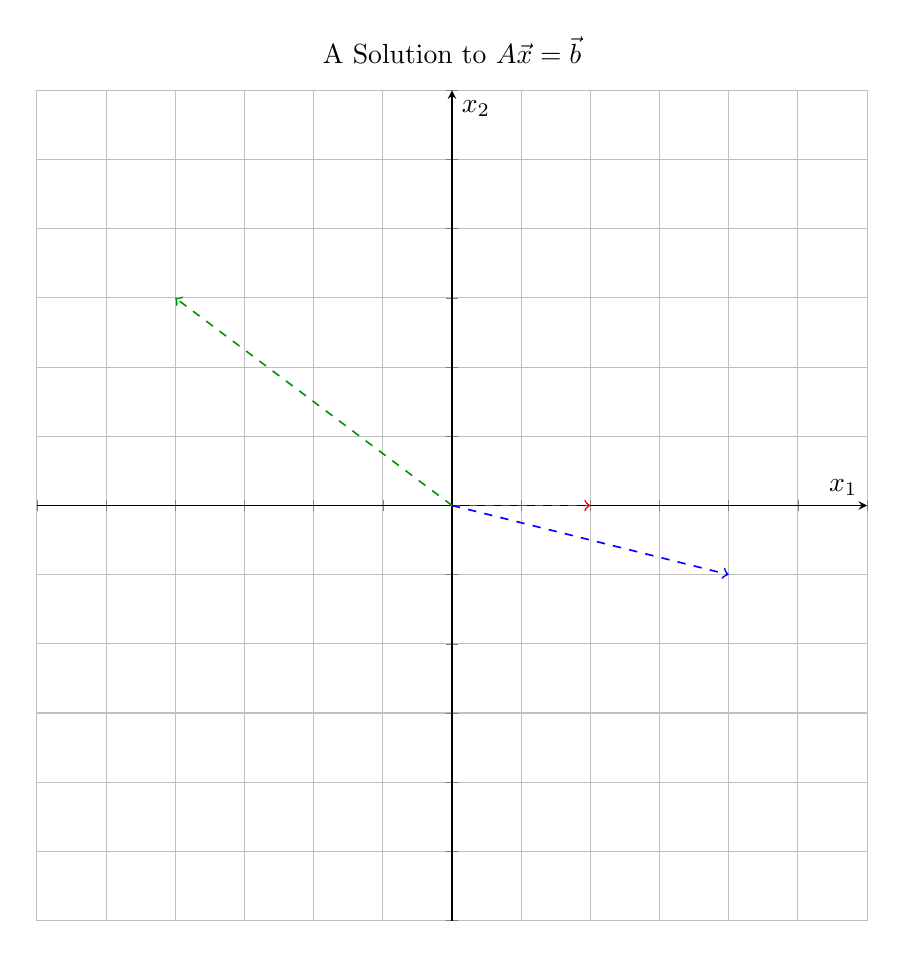
\begin{tikzpicture}
					\begin{axis}[axis lines = middle, grid = major, xmin=-6, xmax=6, ymin=-6, ymax=6, xlabel={\(x_1\)}, ylabel={\(x_2\)},
							   xticklabels=\empty, yticklabels=\empty, xtick distance = 1, ytick distance = 1, title={A Solution to \(A\vec{x}=\vec{b}\)}
							   , height=\textwidth, width=\textwidth]
						\addplot[red, dashed, ->, semithick] coordinates {(0, 0) (2, 0)};
						\addplot[blue, dashed, ->, semithick] coordinates {(0, 0) (4, -1)};
						\addplot[green!60!black, dashed, ->, semithick] coordinates {(0, 0) (-4, 3)};
					\end{axis}
				\end{tikzpicture}
			\end{minipage} & 
			\begin{minipage}{0.25\textwidth}
				\centering
				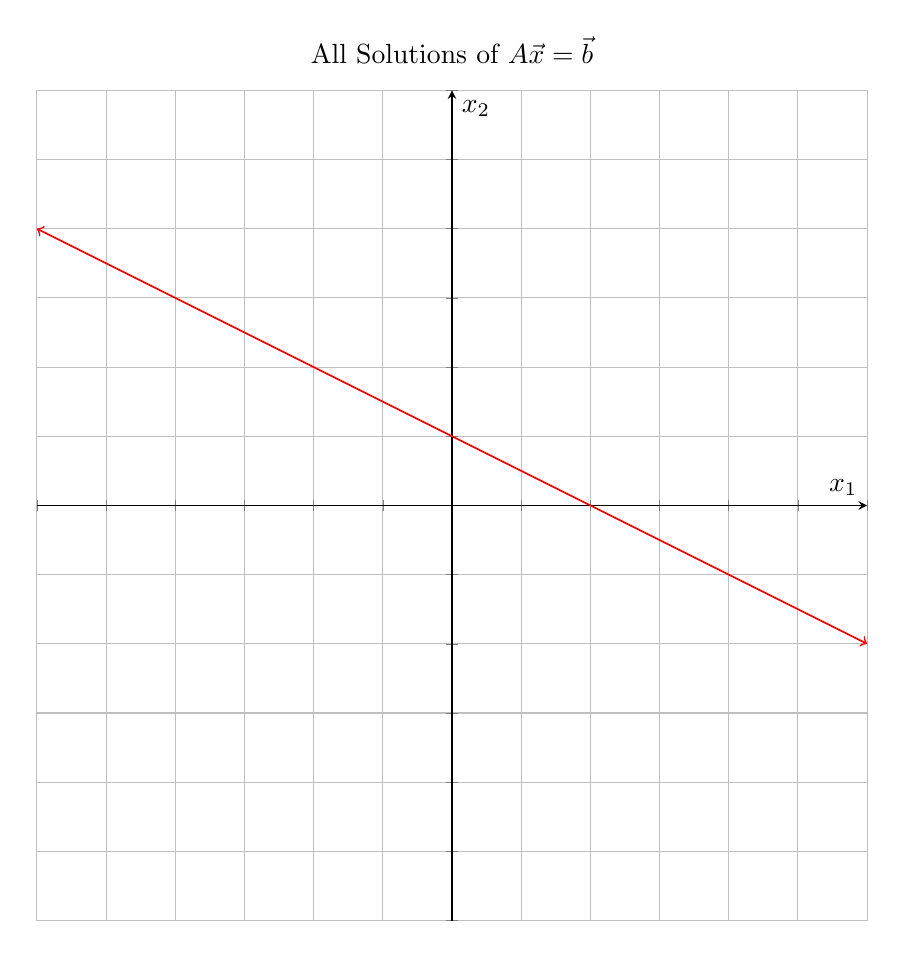
\begin{tikzpicture}
					\begin{axis}[axis lines = middle, grid = major, xmin=-6, xmax=6, ymin=-6, ymax=6, xlabel={\(x_1\)}, ylabel={\(x_2\)},
							   xticklabels=\empty, yticklabels=\empty, xtick distance=1, ytick distance=1, title={All Solutions of \(A\vec{x}=\vec{b}\)}
							   , height=\textwidth, width=\textwidth]
						\addplot[red, <->, semithick, domain=-2:4] ({2 - 2 * x}, {x}); 
					\end{axis}
				\end{tikzpicture}
			\end{minipage} \\
			\begin{minipage}{0.25\textwidth}
				\centering
				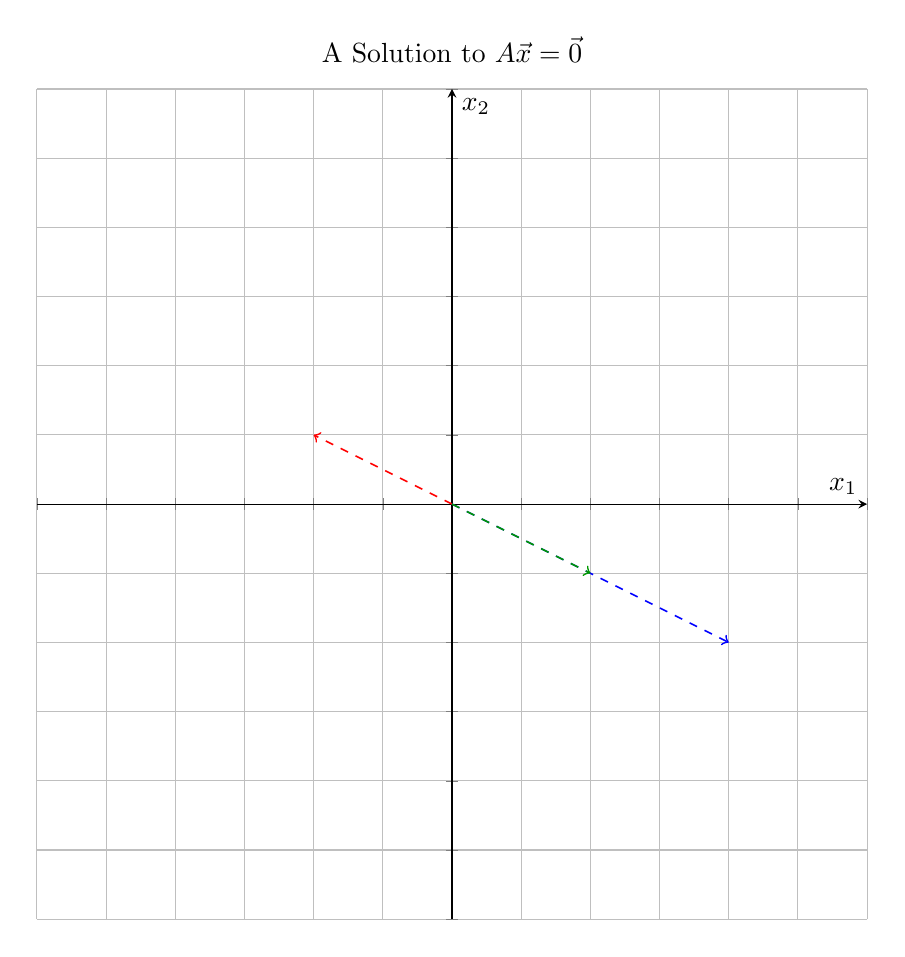
\begin{tikzpicture}
					\begin{axis}[axis lines = middle, grid = major, xmin=-6, xmax=6, ymin=-6, ymax=6, xlabel={\(x_1\)}, ylabel={\(x_2\)},
							   xticklabels=\empty, yticklabels=\empty, xtick distance = 1, ytick distance = 1, title={A Solution to \(A\vec{x}=\vec{0}\)}
							   , height=\textwidth, width=\textwidth]
						\addplot[red, dashed, ->, semithick] coordinates {(0, 0) (-2, 1)};
						\addplot[blue, dashed, ->, semithick] coordinates {(0, 0) (4, -2)};
						\addplot[green!60!black, dashed, ->, semithick] coordinates {(0, 0) (2, -1)};
					\end{axis}
				\end{tikzpicture}
			\end{minipage} &
			\begin{minipage}{0.25\textwidth}
				\centering
				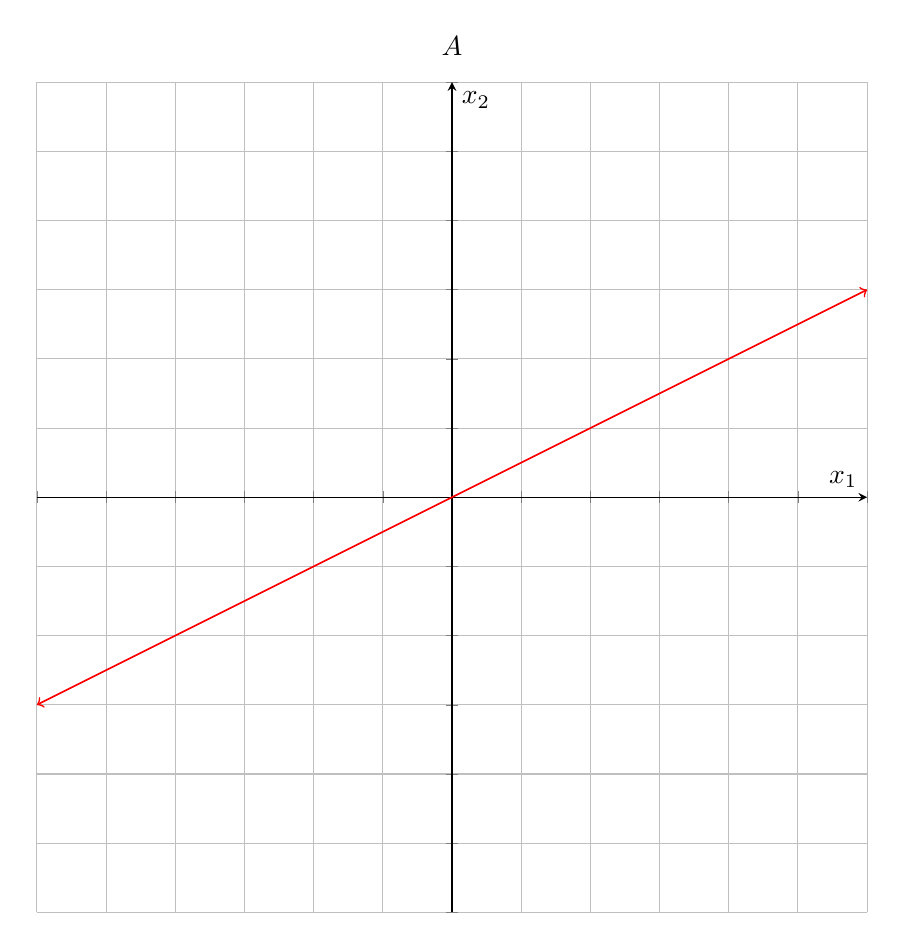
\begin{tikzpicture}
					\begin{axis}[axis lines = middle, grid = major, xmin=-6, xmax=6, ymin=-6, ymax=6, xlabel={\(x_1\)}, ylabel={\(x_2\)},
							   xticklabels=\empty, yticklabels=\empty, xtick distance = 1, ytick distance = 1, title={\(\nullspace A\)}
							   , height=\textwidth, width=\textwidth]
						\addplot[red, <->, semithick, domain=-6:6] {0.5*x};
					\end{axis}
				\end{tikzpicture}
			\end{minipage}\\
			\multicolumn{2}{c}{\begin{minipage}{0.25\textwidth}
				\centering
				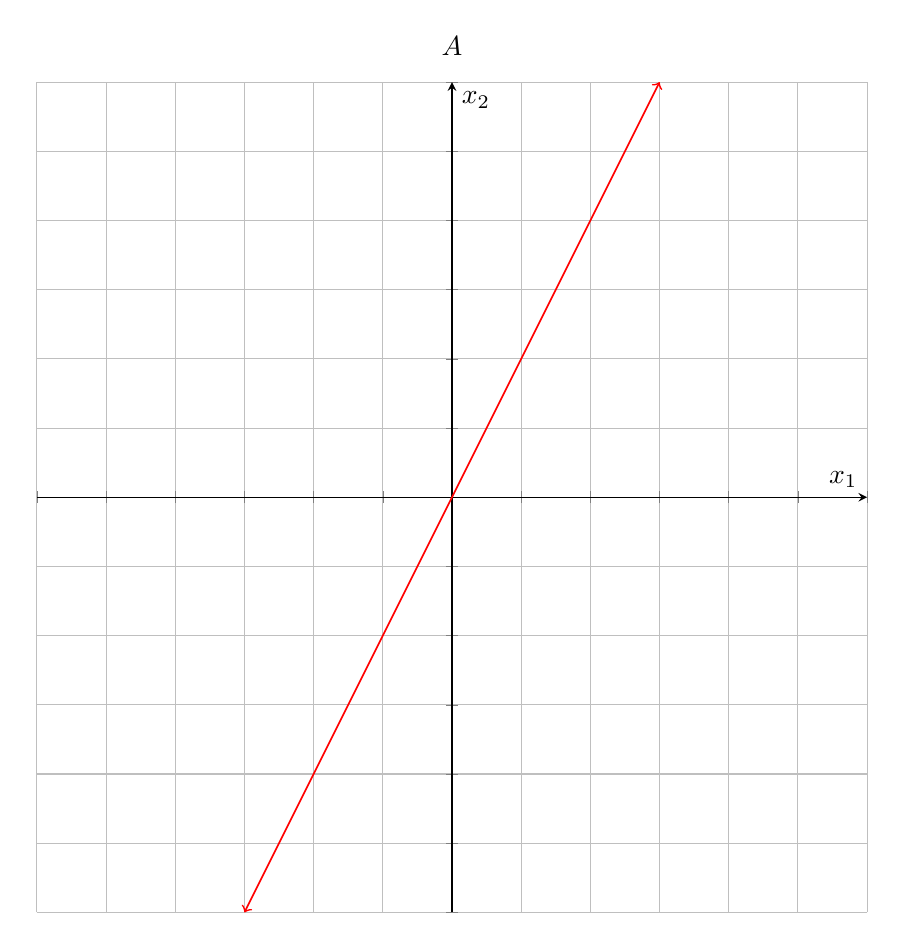
\begin{tikzpicture}
					\begin{axis}[axis lines = middle, grid = major, xmin=-6, xmax=6, ymin=-6, ymax=6, xlabel={\(x_1\)}, ylabel={\(x_2\)},
							   xticklabels=\empty, yticklabels=\empty, xtick distance = 1, ytick distance = 1, title={\(\colspace A\)}
							   , height=\textwidth, width=\textwidth]
						\addplot[red, <->, semithick, domain=-3:3] {2*x};
					\end{axis}
				\end{tikzpicture}
			\end{minipage}}
			\end{tabular}
		\end{figure}
\end{enumerate}